% Options for packages loaded elsewhere
\PassOptionsToPackage{unicode}{hyperref}
\PassOptionsToPackage{hyphens}{url}
%
\documentclass[
  english,
  man,floatsintext]{apa6}
\usepackage{amsmath,amssymb}
\usepackage{lmodern}
\usepackage{ifxetex,ifluatex}
\ifnum 0\ifxetex 1\fi\ifluatex 1\fi=0 % if pdftex
  \usepackage[T1]{fontenc}
  \usepackage[utf8]{inputenc}
  \usepackage{textcomp} % provide euro and other symbols
\else % if luatex or xetex
  \usepackage{unicode-math}
  \defaultfontfeatures{Scale=MatchLowercase}
  \defaultfontfeatures[\rmfamily]{Ligatures=TeX,Scale=1}
\fi
% Use upquote if available, for straight quotes in verbatim environments
\IfFileExists{upquote.sty}{\usepackage{upquote}}{}
\IfFileExists{microtype.sty}{% use microtype if available
  \usepackage[]{microtype}
  \UseMicrotypeSet[protrusion]{basicmath} % disable protrusion for tt fonts
}{}
\makeatletter
\@ifundefined{KOMAClassName}{% if non-KOMA class
  \IfFileExists{parskip.sty}{%
    \usepackage{parskip}
  }{% else
    \setlength{\parindent}{0pt}
    \setlength{\parskip}{6pt plus 2pt minus 1pt}}
}{% if KOMA class
  \KOMAoptions{parskip=half}}
\makeatother
\usepackage{xcolor}
\IfFileExists{xurl.sty}{\usepackage{xurl}}{} % add URL line breaks if available
\IfFileExists{bookmark.sty}{\usepackage{bookmark}}{\usepackage{hyperref}}
\hypersetup{
  pdftitle={Analytical choices for analyzing multidimensional behavior - Many analysts test hypotheses about human speech.},
  pdfauthor={First Author\#, Second Author\#, \ldots\#, \& Last Author\#},
  pdflang={en-EN},
  pdfkeywords={crowdsourcing science, data analysis, scientific transparency, speech, acoustic analysis},
  hidelinks,
  pdfcreator={LaTeX via pandoc}}
\urlstyle{same} % disable monospaced font for URLs
\usepackage{graphicx}
\makeatletter
\def\maxwidth{\ifdim\Gin@nat@width>\linewidth\linewidth\else\Gin@nat@width\fi}
\def\maxheight{\ifdim\Gin@nat@height>\textheight\textheight\else\Gin@nat@height\fi}
\makeatother
% Scale images if necessary, so that they will not overflow the page
% margins by default, and it is still possible to overwrite the defaults
% using explicit options in \includegraphics[width, height, ...]{}
\setkeys{Gin}{width=\maxwidth,height=\maxheight,keepaspectratio}
% Set default figure placement to htbp
\makeatletter
\def\fps@figure{htbp}
\makeatother
\setlength{\emergencystretch}{3em} % prevent overfull lines
\providecommand{\tightlist}{%
  \setlength{\itemsep}{0pt}\setlength{\parskip}{0pt}}
\setcounter{secnumdepth}{5}
% Make \paragraph and \subparagraph free-standing
\ifx\paragraph\undefined\else
  \let\oldparagraph\paragraph
  \renewcommand{\paragraph}[1]{\oldparagraph{#1}\mbox{}}
\fi
\ifx\subparagraph\undefined\else
  \let\oldsubparagraph\subparagraph
  \renewcommand{\subparagraph}[1]{\oldsubparagraph{#1}\mbox{}}
\fi
% Manuscript styling
\usepackage{upgreek}
\captionsetup{font=singlespacing,justification=justified}

% Table formatting
\usepackage{longtable}
\usepackage{lscape}
% \usepackage[counterclockwise]{rotating}   % Landscape page setup for large tables
\usepackage{multirow}		% Table styling
\usepackage{tabularx}		% Control Column width
\usepackage[flushleft]{threeparttable}	% Allows for three part tables with a specified notes section
\usepackage{threeparttablex}            % Lets threeparttable work with longtable

% Create new environments so endfloat can handle them
% \newenvironment{ltable}
%   {\begin{landscape}\begin{center}\begin{threeparttable}}
%   {\end{threeparttable}\end{center}\end{landscape}}
\newenvironment{lltable}{\begin{landscape}\begin{center}\begin{ThreePartTable}}{\end{ThreePartTable}\end{center}\end{landscape}}

% Enables adjusting longtable caption width to table width
% Solution found at http://golatex.de/longtable-mit-caption-so-breit-wie-die-tabelle-t15767.html
\makeatletter
\newcommand\LastLTentrywidth{1em}
\newlength\longtablewidth
\setlength{\longtablewidth}{1in}
\newcommand{\getlongtablewidth}{\begingroup \ifcsname LT@\roman{LT@tables}\endcsname \global\longtablewidth=0pt \renewcommand{\LT@entry}[2]{\global\advance\longtablewidth by ##2\relax\gdef\LastLTentrywidth{##2}}\@nameuse{LT@\roman{LT@tables}} \fi \endgroup}

% \setlength{\parindent}{0.5in}
% \setlength{\parskip}{0pt plus 0pt minus 0pt}

% \usepackage{etoolbox}
\makeatletter
\patchcmd{\HyOrg@maketitle}
  {\section{\normalfont\normalsize\abstractname}}
  {\section*{\normalfont\normalsize\abstractname}}
  {}{\typeout{Failed to patch abstract.}}
\patchcmd{\HyOrg@maketitle}
  {\section{\protect\normalfont{\@title}}}
  {\section*{\protect\normalfont{\@title}}}
  {}{\typeout{Failed to patch title.}}
\makeatother
\shorttitle{Many analysts - one speech data set}
\keywords{crowdsourcing science, data analysis, scientific transparency, speech, acoustic analysis\newline\indent Word count: X}
\usepackage{lineno}

\linenumbers
\usepackage{csquotes}
\usepackage{cleveref}
\usepackage{changes}
\definechangesauthor[name={Stefano Coretta}, color=red]{SC}
\definechangesauthor[name={Timo Röttger}, color=blue]{TR}
\definechangesauthor[name={Joseph Casillas}, color=orange]{JC}
\ifxetex
  % Load polyglossia as late as possible: uses bidi with RTL langages (e.g. Hebrew, Arabic)
  \usepackage{polyglossia}
  \setmainlanguage[]{english}
\else
  \usepackage[main=english]{babel}
% get rid of language-specific shorthands (see #6817):
\let\LanguageShortHands\languageshorthands
\def\languageshorthands#1{}
\fi
\ifluatex
  \usepackage{selnolig}  % disable illegal ligatures
\fi
\newlength{\cslhangindent}
\setlength{\cslhangindent}{1.5em}
\newlength{\csllabelwidth}
\setlength{\csllabelwidth}{3em}
\newenvironment{CSLReferences}[2] % #1 hanging-ident, #2 entry spacing
 {% don't indent paragraphs
  \setlength{\parindent}{0pt}
  % turn on hanging indent if param 1 is 1
  \ifodd #1 \everypar{\setlength{\hangindent}{\cslhangindent}}\ignorespaces\fi
  % set entry spacing
  \ifnum #2 > 0
  \setlength{\parskip}{#2\baselineskip}
  \fi
 }%
 {}
\usepackage{calc}
\newcommand{\CSLBlock}[1]{#1\hfill\break}
\newcommand{\CSLLeftMargin}[1]{\parbox[t]{\csllabelwidth}{#1}}
\newcommand{\CSLRightInline}[1]{\parbox[t]{\linewidth - \csllabelwidth}{#1}\break}
\newcommand{\CSLIndent}[1]{\hspace{\cslhangindent}#1}

\title{Analytical choices for analyzing multidimensional behavior - Many analysts test hypotheses about human speech.}
\author{First Author\textsuperscript{\#}, Second Author\textsuperscript{\#}, \ldots{}\textsuperscript{\#}, \& Last Author\textsuperscript{\#}}
\date{}


\authornote{

Add complete departmental affiliations for each author here. Each new line herein must be indented, like this line.

Enter author note here.

The authors made the following contributions. First Author: Conceptualization, Writing - Original Draft Preparation, Writing - Review \& Editing; Second Author: Writing - Review \& Editing; \ldots{}: Writing - Review \& Editing; Last Author: Writing - Review \& Editing.

Correspondence concerning this article should be addressed to First Author, Postal address. E-mail: \href{mailto:my@email.com}{\nolinkurl{my@email.com}}

}

\affiliation{\vspace{0.5cm}\textsuperscript{1} \#\\\textsuperscript{\ldots{}} \ldots{}}

\abstract{
One or two sentences providing a \textbf{basic introduction} to the field, comprehensible to a scientist in any discipline.

Two to three sentences of \textbf{more detailed background}, comprehensible to scientists in related disciplines.

One sentence clearly stating the \textbf{general problem} being addressed by this particular study.

One sentence summarizing the main result (with the words ``\textbf{here we show}'' or their equivalent).

Two or three sentences explaining what the \textbf{main result} reveals in direct comparison to what was thought to be the case previously, or how the main result adds to previous knowledge.

One or two sentences to put the results into a more \textbf{general context}.

Two or three sentences to provide a \textbf{broader perspective}, readily comprehensible to a scientist in any discipline.
}



\begin{document}
\maketitle

\hypertarget{introduction}{%
\section{Introduction}\label{introduction}}

In order to effectively accumulate knowledge, science needs to (i) produce data that can be replicated using the original methods and (ii) arrive at robust conclusions substantiated by the data.
In recent coordinated efforts to replicate published findings, the scientific disciplines have uncovered surprisingly low success rates for (i) (Camerer et al., 2018; e.g., Open Science Collaboration, 2015) leading to what is now referred to as the \emph{replication crisis}.
Beyond the difficulties of replicating scientific findings, a growing body of evidence suggests that the theoretical conclusions drawn from data are often variable even when researchers have access to reliable data (REFS).
The latter situation has been referred to as the \emph{inference crisis} (Rotello, Heit, \& Dubé, 2015; Starns et al., 2019) and is, among other things, rooted in the inherent flexibility of data analysis (Gelman \& Loken, 2014; often referred to as researcher degrees of freedom: Simmons, Nelson, \& Simonsohn, 2011).
Data analysis involves many different steps, such as inspecting, organizing, transforming, and modeling the data, to name a few.
Along the way, different methodological and analytical choices need to be made, all of which may influence the final interpretation of the data.
These researcher degrees of freedom are both a blessing and a curse.

They are a blessing because they afford us the opportunity to look at nature from different angles, which, in turn, allows us to make important discoveries and generate new hypothesis (e.g., Box, 1976; De Groot, 2014; Tukey, 1977).
They are a curse because idiosyncratic choices can lead to categorically different interpretations, which eventually find their way into the publication record where they are taken for granted (Simmons, Nelson, \& Simonsohn, 2011).
Recent projects have shown that the variability between different data analysts is vast.
This variability can lead independent researchers to draw different conclusions about the same data set as demonstrated by several projects crowd-sourcing analysis strategies (Botvinik-Nezer et al., 2020; e.g., Silberzahn et al., 2018; Starns et al., 2019).
These projects, however, might still underestimate the extent to which analysts vary because data analysis is not merely restricted to statistical inference.
Human behavior is complex and offers many ways to be translated into numbers.
This is particularly true for fields that draw conclusions about human behavior and cognition from multidimensional data like audio or video data.
In fields working on human speech production, for example, researchers need to make numerous decisions about what to measure and how to measure it.
This is not trivial given the temporal extension of the acoustic signal and its complex structural composition.
Not only can decisions about measuring the signal influence downstream decisions about statistical modeling, but statistical results or modeling issues can also lead researchers to go back and revise earlier decisions about the measuring process itself.

In this article, we investigate the variability in analytic choices when many analyst teams analyze the same speech production data, a process that involves both decisions regarding the operationalization of a complex observed signal and decisions regarding the statistical modeling.
Specifically, we report the impact of the analytic pipeline on research results obtained by XX teams who gained access to the same set of acoustic recordings in order to answer the same research question.

\hypertarget{researcher-degrees-of-freedom}{%
\subsection{Researcher degrees of freedom}\label{researcher-degrees-of-freedom}}

Data analysis comes with many decisions like how to measure a given phenomenon or behavior, what data to submit to statistical modeling and which to exclude in the final analysis, or what inferential decision procedure to apply.
However, if these decisions during data analysis are not specified in advance, we might stumble upon seemingly meaningful patterns in the data that are merely statistical flukes.
This can be problematic because humans show cognitive biases that can lead to erroneous inferences.
Humans filter the world in irrational ways (e.g., Tversky \& Kahneman, 1974), seeing coherent patterns in randomness (Brugger 2001), convincing themselves of the validity of prior expectations ({``I knew it,''} Nickerson, 1998), and perceiving events as being plausible in hindsight ({``I knew it all along,''} Fischhoff, 1975).
In connection with an academic incentive system that rewards certain discovery processes more than others (Koole \& Lakens, 2012; Sterling, 1959), we often find ourselves exploring many possible analytical pipelines, but only reporting a select few.
This issue is particularly amplified in fields in which the raw data lend themselves to many possible ways to measure (Roettger, 2019).
Combined with a wide variety of methodological and theoretical traditions as well as varying levels of statistical training across subfields, the inherent flexibility of data analysis might lead to a vast plurality of analytic approaches that can lead to different scientific conclusions.
Consequently, there might be many published papers that present overconfident interpretations of their data based on idiosyncratic analytic strategies (Gelman \& Loken, 2014; e.g., Simmons, Nelson, \& Simonsohn, 2011).
These interpretations are either associated with an unknown amount of uncertainty or lend themselves to alternative interpretation if analyzed differently.
However, instead of being critically evaluated, scientific results often remain unchallenged in the publication record.
Despite recent efforts to improve transparency and reproducibility (REFS) and freely available and accessible infrastructures such as provided by the Open Science Framework (osf.io, ADD), critical re-analyses of published analytic strategies are still not very common because data sharing remains rare (Wicherts, Borsboom, Kats, \& Molenaar, 2006).

While this issue has been widely discussed both from a conceptual point of view (Nosek \& Lakens, 2014; Simmons, Nelson, \& Simonsohn, 2011; Wagenmakers, Wetzels, Borsboom, Maas, \& Kievit, 2012) and its application in individual scientific fields (e.g.~Wichert et al.~2015, Charles et al.~2019, Roettger, 2019), there are still many unknowns regarding the extent of analytical plurality in practice.
Recent collaborative attempts have started to shed light on how different analysts tackle the same data set and have revealed a large amount of variability.

\hypertarget{crowdsourcing-alternative-analyses}{%
\subsection{Crowdsourcing alternative analyses}\label{crowdsourcing-alternative-analyses}}

In a collaborative effort, Silberzahn et al. (2018) let twenty-nine independent analysis teams address the same research hypothesis.
Analytical approaches and consequently the results varied widely between teams.
Sixty-nine percent of the teams found support for the hypothesis, and 31\% did not.
Out of the 29 analytical strategies, there were 21 unique combinations of covariates.
Importantly, the observed variability was neither predicted by the team's preconceptions about the phenomenon under investigation nor by peer ratings of the quality of their analyses.
The authors results suggest that analytic plurality is a fact of life and not driven by different levels of expertise or bias.
Similar crowd-sourced studies recruiting independent analyst teams showed similar results.

While these projects show a large degree of analytical flexibility with impactful consequences, they dealt with flexibility in inferential or computational modeling.
In these studies the data sets were fixed and data collection or measurement could not be changed.

However, in many fields the primary raw data are complex signals that need to be operationalized according to the research question.
In social sciences, the raw observations correspond to human behavior, sometimes measured as a complex visual or acoustic signal.
Decisions about how to measure a theoretical construct related to that behavior or its underlying cognitive processes might interact with downstream decisions about statistical modeling and vice versa (Flake \& Fried, 2019).
To understand how analytical flexibility manifests itself in a scenario where a complex decision procedure is involved in operationalizing and measuring complex signals, the present paper looks at an experimentally elicited speech data set.

\hypertarget{operationalizing-speech}{%
\subsection{Operationalizing speech}\label{operationalizing-speech}}

Research on speech is at the heart of the cognitive sciences, informing psychological models of language, categorization, and memory, guiding methods for diagnosis and therapy of speech disorders, and facilitating advancement in automatic speech recognition and speech synthesis. One major challenge in the speech sciences is the mapping between communicative intentions and their physical manifestation.

Speech is a complex signal that is characterized by structurally different acoustic landmarks distributed throughout different temporal domains.
Thus, choosing how to measure a phenomenon of interest is an important and non-trivial analytical decision. Take for example the following sentence in 1:

\begin{enumerate}
\def\labelenumi{(\arabic{enumi})}
\tightlist
\item
  ``I can't bear another meeting on zoom.''
\end{enumerate}

Depending on the speaker's intention, this sentence can be said in different ways.
If, for instance, the speaker is exhausted by all their meetings, the speaker might acoustically highlight the word ``another'' or ``meeting.''
If, on the other hand, the speaker is just tired of video conferences, they might acoustically highlight the word ``zoom.''

If we want to compare the speech signal associated with these two intentions, how do we quantify the difference between them? What do we measure and how do we measure it?
Given the continuous and transient nature of speech, identifying speech parameters and temporal domains becomes a non-trivial task.
Utterances stretch over hundreds of milliseconds and contain several levels of linguistically relevant units such as phrases, words, syllables, and individual sounds.
The researcher is thus confronted with a considerable number of parameters and combinations thereof to choose from.

Speech categories are inherently multidimensional and dynamic: they consist of a cluster of parameters that are modulated over time.
The acoustic parameters of one category are usually asynchronous, i.e.~they appear at different time points in the unfolding signal, and overlap with parameters of other categories {[}e.g., Jongman, Wayland, and Wong (2000); Lisker (1986); Summerfield, 1984; Winter (2014){]}.
A classical example is the distinction between voiced and voiceless stops in English (i.e.~/b/ and /p/ in \emph{bear} vs \emph{pear}).
This voiced/voiceless contrast is manifested by many acoustic features which can differ depending on several factors, such as position of the consonant in the word and surrounding sounds (Lisker, 1977).
Furthermore, correlates of the contrast can even be found away from the consonant, in temporally distant speech units.
For example, the initial /l/ of the English words \emph{led} and \emph{let} is affected by the voicing of the final consonant (/t, d/) (Hawkins \& Nguyen, 2004).
The multiplicity of phonetic cues grows exponentially if we look at larger temporal domains as is the case for suprasegmental aspects of speech.
For example, studies investigating acoustic correlates of word stress (e.g.~the difference between \emph{insíght} and \emph{íncite}) have been using a wide variety of measurements, including temporal characteristics (duration of certain segments or sub-segmental intervals), spectral characteristics (intensity, formants, and spectral tilt), and measurements related to fundamental frequency (f0) (e.g., Gordon \& Roettger, 2017).

Moving onto the expression of higher-level functions like information structure and discourse pragmatics, relevant acoustic cues can be distributed throughout even larger domains, such as phrases and whole utterances (e.g., Ladd, 2008).
Differences in position, shape, and alignment of pitch modulations over multiple locations within a sentence are correlated with differences in discourse functions (e.g.~Niebuhr et al., 2011).
The latter can also be expressed by global vs local pitch modulations (Haan 2002), as well as acoustic information within the temporal or spectral domain (e.g., Van Heuven \& Van Zanten, 2005).
Extra-linguistic information, like speaker's intentions, levels of arousal or social identity, are also conveyed by broad-domain parameters, such as voice quality, rhythm, and pitch (Foulkes \& Docherty, 2006; Ogden, 2004; White, Payne, \& Mattys, 2009).

When testing hypotheses on speech production data, researchers are faced with many choices and possibilities.
The larger the functional domain (e.g.~segments vs words vs utterances), the higher the number of conceivable operationalizations.
For example, when comparing two realization of example (1) (here repeated as 2), one of which is intended to signal emphasis on \emph{another} and one of which emphasizes \emph{zoom}.

(2a) ``I can't bear ANOTHER meeting on zoom.''\\
(2b) ``I can't bear another meeting on ZOOM.''

In text ref to Figure \ref{fig:forkingPaths}



\begin{figure}
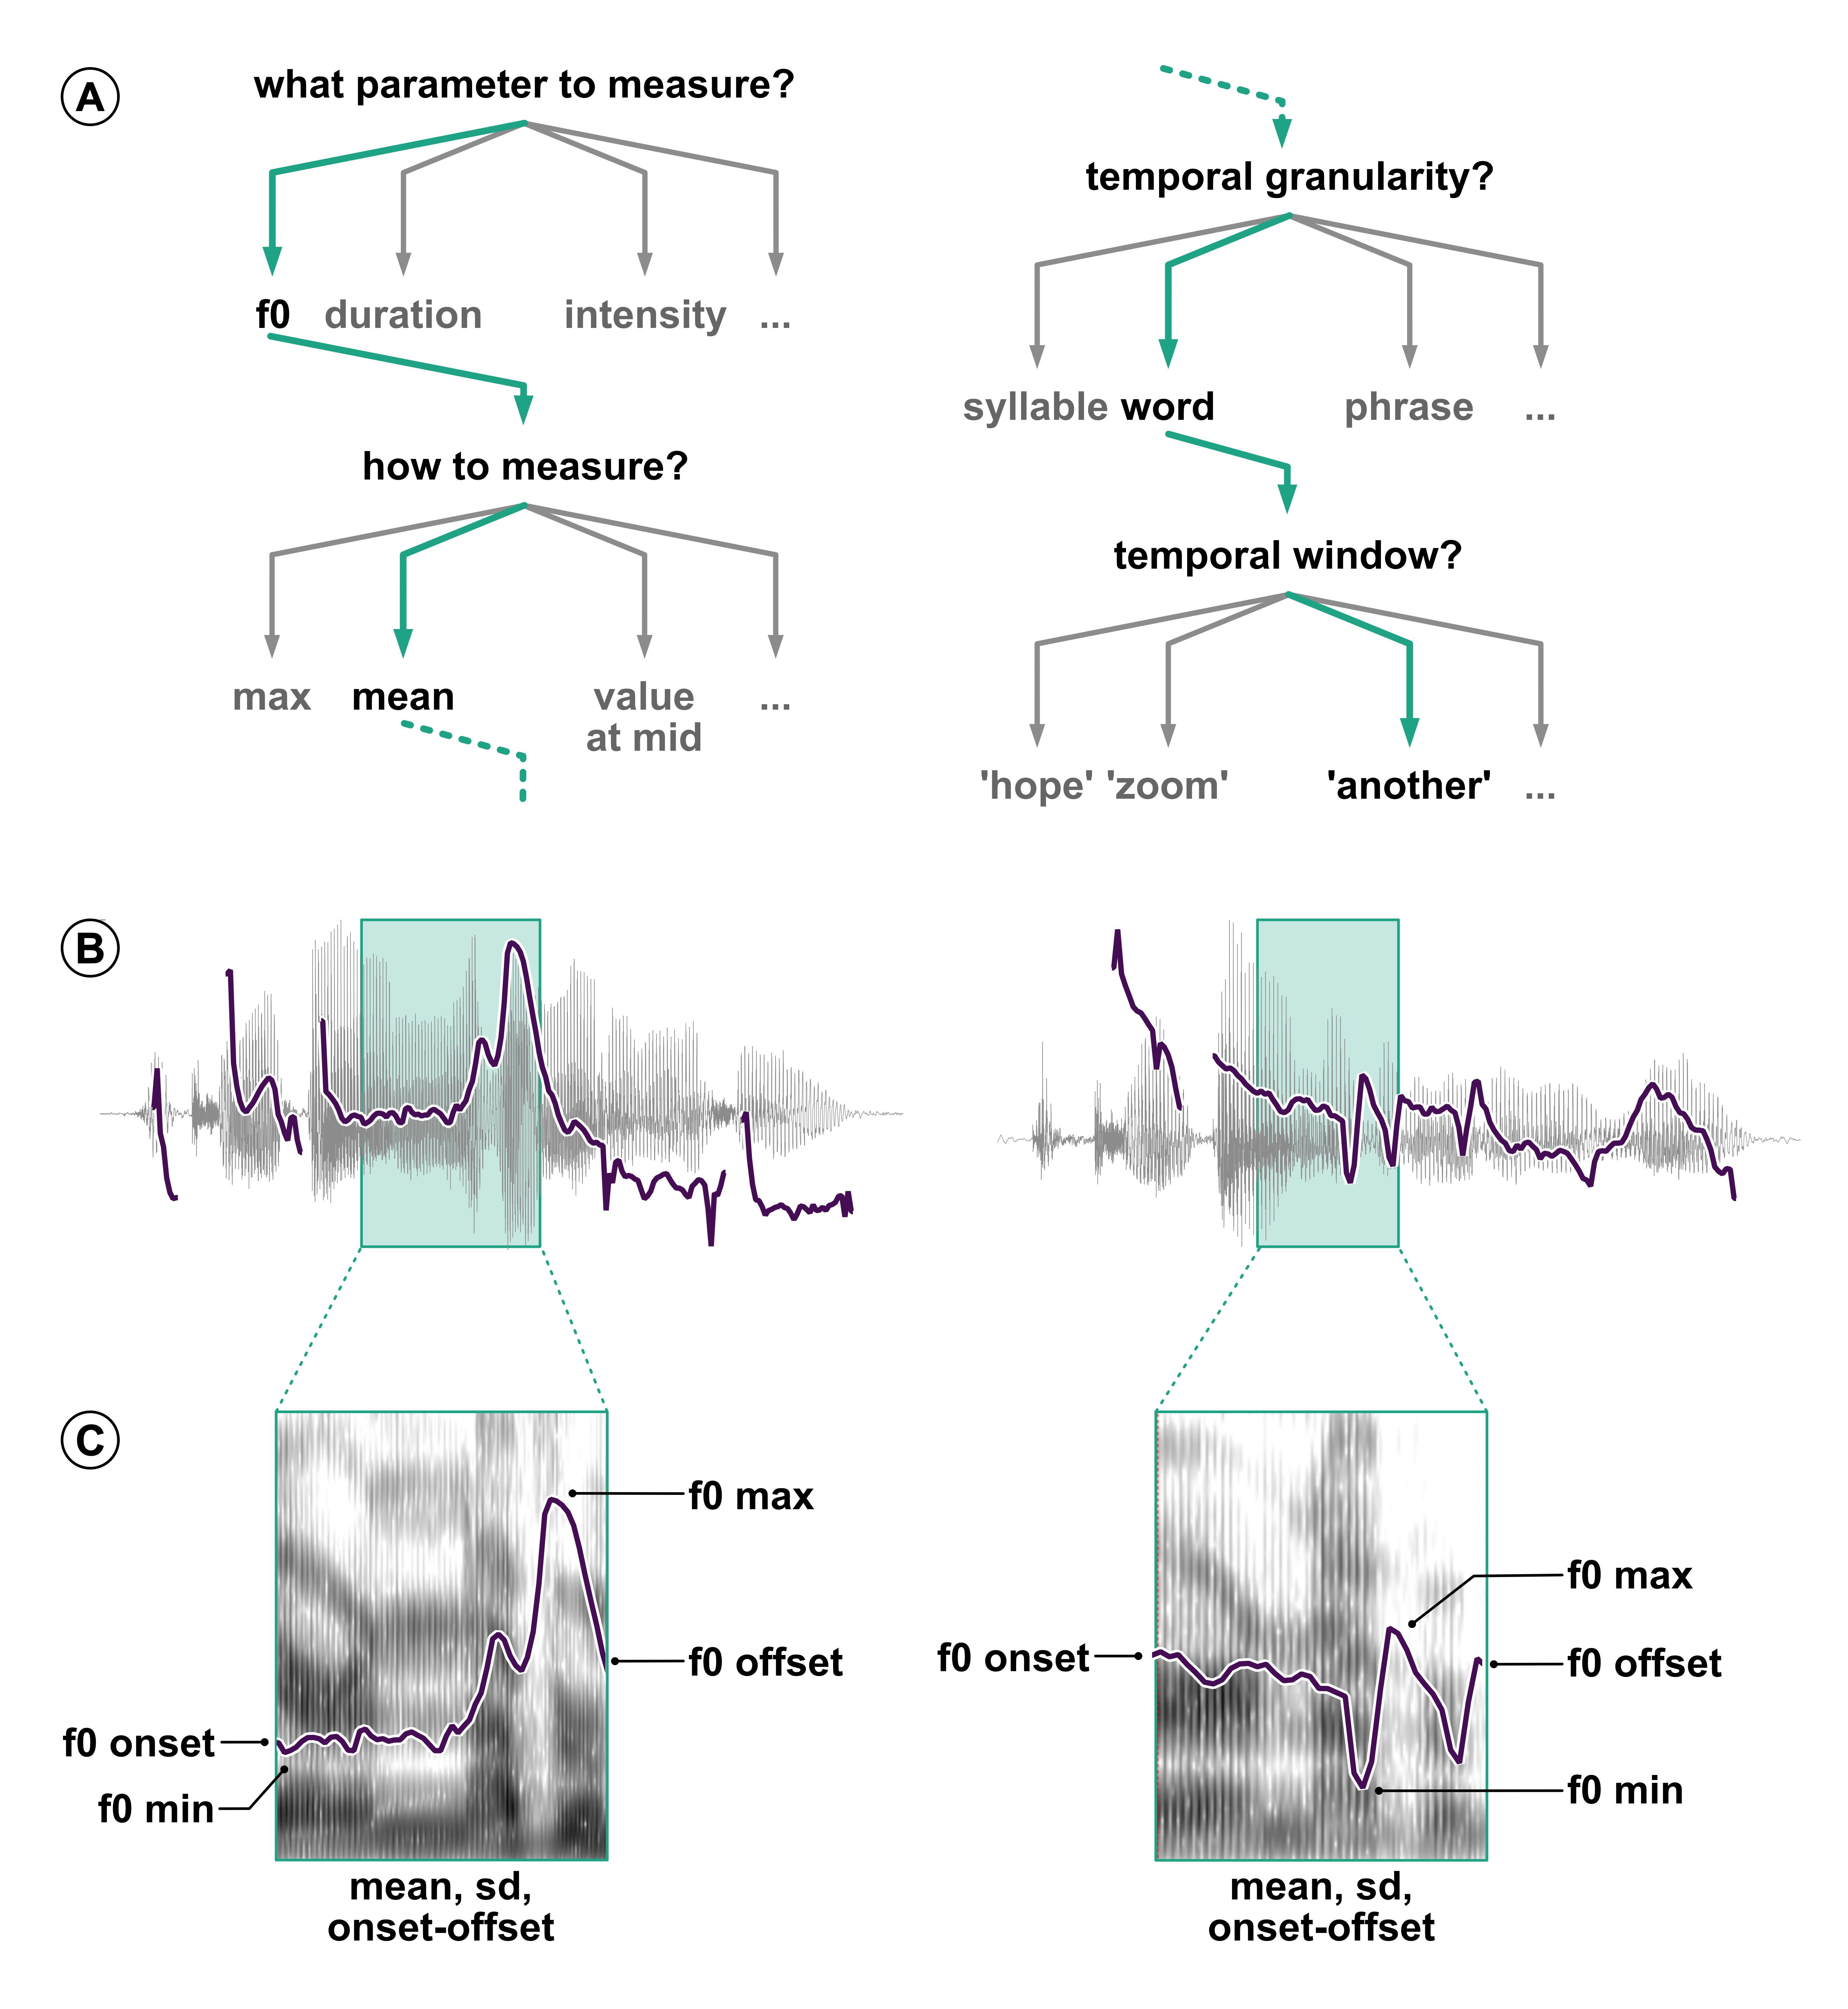
\includegraphics[width=1\linewidth]{/Users/ste/repos/many_analyses/figs/ForkingPaths} \caption{Illustrations of the analytical flexibility associated with acoustic analyses. (A) an example of multiple possible and justifiable decisions when comparing to utterances; (B) waveform and fundamental frequency (f0) track of two instances of utterances 2a and 2b. The words ``another is highlighted by the green box'\,'; (C) spectrogram and f0 track of the word another, exemplifying different operationalizations of differences in pitch.}\label{fig:forkingPaths}
\end{figure}

Do we only compare the word \emph{another} in 2a and 2b or also the word \emph{zoom} or do we measure utterance wide acoustic profiles? Do we measure the whole word? Or just the stressed syllable?
Do we average the domain or do we measure a specific point in time?
Do we measure fundamental frequency or intensity?
When looking at phrase-wide temporal domains, the number of possible analytical pipelines quickly explodes.
This plurality of analytical paths is illustrated in figure X.
When comparing two utterance such as 2a and 2b, there are many things to consider.
Even if we know that we want to compare fundamental frequency of only the word \emph{another} across utterances 2a and 2b, there are still many decisions to be made, all of which can be justified.
For example, we could measure f0 at specific points in time like the onset of the window, the offset, the midpoint.
We could also measure the value or time of the minimum or maximum f0 value.
We could summarise f0 across the entire window and extract the mean, median or standard deviation of f0.
And the garden of forking paths does not stop here.
In Figure X, we went with a specific option to automatically calculate f0, INSERT SOME EXAMPLES OF PITCH TRACKING OPTIONS.
Moreover, knowing that theses estimates are somewhat noisy, we could smooth these contours to different degrees, automatically or manually remove estimates that are off, etc.

These decisions are usually made prior to any statistical analysis, but are at times revised a posteriori (i.e.~after data collection and/or preliminary analyses) in light of unforeseen or surprising outcomes.
These myriads of possible decisions are exponentiated by researcher degrees of freedom related to statistical analysis (e.g.~Wicherts et al.~????).
Even the analysis of a single measure can be approached via an ever-increasing range of different statistical models (REFs).
The present paper probes this garden of forking paths in the analysis of speech.
To assess the variability in data analysis pipelines across independent researchers, we provided XX analytical teams with an experimentally elicited speech corpus and asked them to investigate acoustic differences related to a functional contrast that might be manifested across the whole utterance.

\hypertarget{the-data-set---the-prosody-of-redundant-modifiers}{%
\subsection{The data set - The prosody of redundant modifiers}\label{the-data-set---the-prosody-of-redundant-modifiers}}

Our data set was collected in order to answer the following research question: Do speakers acoustically modify utterances to signal atypical word combinations? (e.g.~\emph{a blue banana} vs \emph{a yellow banana})?
We are interested in the acoustic profile of referring expressions.
Referring is one of the most basic and prevalent uses of language and one of the most widely researched areas in language science.
It is an open question how speakers choose a referring expression when they want to refer to a specific entity like a banana.
The context within which an entity occurs (i.e., with other non-fruits, other fruits, or other bananas) plays a large part in determining the choice of referring expressions.
Generally, speakers aim to be as informative as possible to uniquely establish reference to the intended object, but they are also resource-efficient in that they avoid redundancy (Grice, 1975).
Thus one would expect the use of a modifier, for example, only if it is necessary for disambiguation.
For instance, one might use the adjective \emph{yellow} to describe a banana in a situation in which there is a yellow and a less ripe green banana available, but not when there is only one banana to begin with.

Despite this coherent idea that speakers are both rational and efficient, there is much evidence that speakers are often over-informative: Speakers use referring expressions that are more specific than strictly necessary for the unambiguous identification of the intended referent (Rubio-Fernández, 2016; Sedivy, 2003; Westerbeek, Koolen, \& Maes, 2015), which has been argued to facilitate object identification and making communication between speakers and listeners more efficient (Arts, Maes, Noordman, \& Jansen, 2011; Paraboni, Van Deemter, \& Masthoff, 2007; Rubio-Fernández, 2016).
Recent findings suggest that the utility of a referring expression depends on how good it is for a listener (compared to other referring expressions) to identify a target object.
For example, Degen, Hawkins, Graf, Kreiss, and Goodman (2020) showed that modifiers that are less typical for a given referent (e.g.~a blue banana) are more likely to be used in an over-informative scenario (e.g.~when there is just one banana).
This account, however, has mainly focused on content selection (Gatt, Gompel, Deemter, \& Krahmer, 2013), i.e.~whether a certain referential expression is chosen or not, ignoring the fact that speech communication is much richer.

Even looking at morphosyntactically identical expressions, speakers can modulate these via suprasegmental acoustic properties like temporal and spectral modifications of the segments involved (e.g., Ladd, 2008).
Most prominently, languages use intonation to signal discourse relationships between referents (among other functions).
Intonation marks discourse-relevant referents for being new or given information to guide the listeners' interpretation of incoming messages.
In many languages, speakers can use particular pitch movements to signal whether a referent has already been mentioned and is therefore referred back to, or a referent is newly introduced into the discourse.
Many languages use intonation in order to signal if a referent is contrasting with one or more alternatives that are relevant to the current discourse.
Content selection aside, in a scenario in which a speaker wants to refer to a banana when there is also a pear on the table, the speaker would most likely produce a high rising pitch accent on \emph{banana} to indicate the contrastive nature of the noun.
In a scenario in which the speaker wants to refer to a yellow banana when there is also a less ripe green banana on the table, the speaker would most likely produce a high rising pitch accent on \emph{yellow} to indicate the contrastive nature of the modifier.
In addition to a pitch accent, elements that are new and/or contrastive are often produced with additional suprasegmental prominence, i.e.~segments are hyperarticulated, resulting in longer, louder and more clearly articulated acoustic targets.

\hypertarget{research-questions}{%
\subsection{Research questions}\label{research-questions}}

The present project examines the extent to which subjective choices by different researchers analyzing a complex speech data set affect the reported results.
We are further interested in which factors affect the researchers' final results.

\hypertarget{methods}{%
\section{Methods}\label{methods}}

We are closely following the methodology proposed by Parker et al.~(Stage 1 in-principle accepted) in terms of data collection.
However, the analysis will substantially diverge from their approach (see §\#.\#)

This project involves a series of steps (X-X):

\begin{enumerate}
\def\labelenumi{\arabic{enumi}.}
\tightlist
\item
  We will recruit independent groups of researchers to analyze the data.
\item
  We will give researchers access to the speech corpus and let them analyze the data as they see fit.
\item
  We will ask reviewers to generate peer review ratings of the analyses based on methods (not results).
\item
  We will evaluate the variation among the different analyses.
\item
  Lastly, we will collaboratively produce the final manuscript.
\end{enumerate}

We estimate that this process, from the time of an in-principle acceptance of this Stage 1 Registered Report, will take XX months (Table X).
The factor most likely to delay our time line is the rate of completion of the original set of analyses by independent groups of scientists.

\hypertarget{step-1-recruitment-and-initial-survey-of-analysts}{%
\subsection{Step 1: Recruitment and Initial Survey of Analysts}\label{step-1-recruitment-and-initial-survey-of-analysts}}

The initiating authors (SC, JC, TR) created a publicly available document providing a general description of the project (LINK) and a short prerecorded slide show that summarizes the study and research question in order to increase accessibility to potential analysts (LINK).
The project will be advertised via Social Media, using mailing lists for linguistic and psychological societies (full scope of these lists is not fixed but will include LIST OF LISTS), and via word of mouth.
The target population is active speech science researchers with a graduate degree (or currently studying for a graduate degree) in a relevant discipline.
Researchers can choose to work independently or in a small team.
For the sake of simplicity, we refer to single researcher or small teams as ``analysis teams.''

Recruitment for this project is ongoing but we aim for a minimum of XX analysis teams independently evaluating each data set (see sample size justification below).
We will simultaneously recruit volunteers to peer-review the analyses conducted by the other volunteers through the same channels.
Our goal is to recruit a similar number of peer-reviewers and analysts, and to ask each peer reviewer to review a minimum of four analyses.
If we are unable to recruit at least half the number of reviewers as analysis teams, we will ask analysts to serve also as reviewers (after they have completed their analyses).
All analysts and reviewers will share co-authorship on this manuscript and will participate in the collaborative process of producing the final manuscript.
All analysts will sign a consent (ethics) document (LINK).

To identify the minimal sample size, we followed the method in {[}ECO RR{]}.
The aim of the meta-analysis is to obtain an estimate of heterogeneity of the effect sizes reported by the analysis teams (\(\tau^2\), i.e.~the variance \(\sigma^2_{\alpha_{\text{team}}}\), see \Cref{s:meta-est}).
Ideally, the 95\% credible interval (CrI) of \(\tau^2\) should not include 0 (i.e.~the probability \(p\) that the 95\% CrI contains 0 should be less than 0.05).
The probability \(p\) that a CrI interval does not include 0 is obtained via the \emph{t}-statistics:

\[t = \frac{\tau^2}{SE(\tau^2)}\]

Assuming that the underlying distribution of effect sizes is normal (Knight, 2000), the standard error of \(\tau^2\) can be calculated with the formula:

\[SE(\tau^2) = \sqrt{\frac{2\tau^4}{(n-1)}}\]

where \(n\) is the sample size.
Since we know \(p\) and \(\tau^2\), we can calculate \(n\) such that \(p < 0.05\).
Plugging \(SE(\tau^2)\) into the formula of the \emph{t}-statistics shows that, when \(n\) is fixed, \emph{t} (and hence \(p\)) will be the same regardless of \(\tau^2\):

\[t = \frac{\tau^2}{SE(\tau^2)} = \frac{\tau^2}{\sqrt{\frac{2\tau^4}{(n-1)}}} = \sqrt{\frac{(n-1)}{2}}\]

In other words, the minimum sample size \(n\) needed to exclude 0 from the 95\% CrI of \(\tau^2\) is invariant regardless of the estimate of heterogeneity \(\tau^2\).
When \(n = 12\) then \(t_{(12-1)} = t_{(11)} = 2.3452\) and \(p = 0.0388\), which is below the 0.05 threshold, as required.
In sum, a minimal sample of 12 effect sizes (i.e.~of 12 analysis teams) would thus be sufficient to exclude 0 from the 95\% CrI of \(\tau^2\).

\hypertarget{step-2-primary-data-analyses}{%
\subsection{Step 2: Primary Data Analyses}\label{step-2-primary-data-analyses}}

The analysis teams will register and answer a demographic and expertise survey (LINK).
The survey collects information on the analysts current position and self-estimated breadth and level of statistical expertise.
We will then provide teams with the acoustic data set and request that they answer the following research question:

Do speakers acoustically modify utterances to signal atypical word combinations?

Once their analysis is complete, they will answer a structured survey (LINK), providing analysis technique, explanations of their analytical choices, quantitative results, and a statement describing their conclusions.
They will also upload their analysis files (including the additionally derived data and text files that were used to extract and pre-process the acoustic data), their analysis code (if applicable), and a detailed journal-ready statistical methods section.

\hypertarget{step-3-peer-reviews-of-analyses}{%
\subsection{Step 3: Peer Reviews of Analyses}\label{step-3-peer-reviews-of-analyses}}

At a minimum, each analysis will be evaluated by four different reviewers, and each volunteer peer-reviewer will be randomly assigned to methods sections from at least four analyst teams (the exact number will depend on the number of analysis teams and peer reviewers recruited).
Each peer reviewer will register and answer a demographic and expertise survey identical to that asked of the analysts.
Reviewers will evaluate the methods of each of their assigned analyses one at a time in a sequence determined by the initiating authors.
The sequences will be systematically assigned so that, if possible, each analysis is allocated to each position in the sequence for at least one reviewer.
For instance, if each reviewer is assigned four analyses to review, then each analysis will be the first analysis assigned to at least one reviewer, the second analysis assigned to another reviewer, the third analysis assigned to yet another reviewer, and the fourth analysis assigned to a fourth reviewer.
Balancing the order in which reviewers see the analyses controls for order effects, e.g.~a reviewer might be less critical of the first methods section they read than the last.
The process for a single reviewer will be as follows.
First, the reviewer will receive a description of the methods of a single analysis.
This will include the narrative methods section, the analysis team's answers to our survey questions regarding their methods, including analysis code, and the data set.
The reviewer will then be asked, in an online survey (LINK), to rate both the acoustic analysis and the statistical analysis on a scale of 0-100 based on these prompts:

"Rate the overall appropriateness of the acoustic analysis to answer the research question with the available data. To help you calibrate your rating, please consider the following guidelines:

\begin{itemize}
\item
  \begin{enumerate}
  \def\labelenumi{\arabic{enumi}.}
  \setcounter{enumi}{99}
  \tightlist
  \item
    A perfect analysis with no conceivable improvements from the reviewer.
  \end{enumerate}
\item
  \begin{enumerate}
  \def\labelenumi{\arabic{enumi}.}
  \setcounter{enumi}{74}
  \tightlist
  \item
    An imperfect analysis but the needed changes are unlikely to dramatically alter final interpretation.
  \end{enumerate}
\item
  \begin{enumerate}
  \def\labelenumi{\arabic{enumi}.}
  \setcounter{enumi}{49}
  \tightlist
  \item
    A flawed analysis likely to produce either an unreliable estimate of the relationship or an over-precise estimate of uncertainty.
  \end{enumerate}
\item
  \begin{enumerate}
  \def\labelenumi{\arabic{enumi}.}
  \setcounter{enumi}{24}
  \tightlist
  \item
    A flawed analysis likely to produce an unreliable estimate of the relationship and an over-precise estimate of uncertainty.
  \end{enumerate}
\item
  \begin{enumerate}
  \def\labelenumi{\arabic{enumi}.}
  \setcounter{enumi}{-1}
  \tightlist
  \item
    A dangerously misleading analysis, certain to produce both an estimate that is wrong and a substantially over-precise estimate of uncertainty that places undue confidence in the incorrect estimate.
  \end{enumerate}
\end{itemize}

*Please note that these values are meant to calibrate your ratings.
We welcome ratings of any number between 0 and 100."

After providing this rating, the reviewer will then be shown a series of text boxes and the following prompts:

\noindent ``Please explain your ratings of this analysis.
\noindent Please evaluate the selection of acoustic features.
\noindent Please evaluate the measurement of acoustic features.
\noindent Please evaluate the choice of statistical analysis type.
\noindent Please evaluate the process of choosing variables and structuring of the statistical model.
\noindent Please evaluate the suitability of the variables included in (or excluded from) the statistical model.
\noindent Please evaluate the suitability of the structure of the statistical model.
\noindent Please evaluate choices to exclude or not exclude subsets of the data.
\noindent Please evaluate any choices to transform data (or, if there were no transformations, but you think there should have been, please discuss that choice).''

After submitting this review, a methods section from a second analysis will then be made available to the reviewer.
This same sequence will be followed until all analyses allocated to a given reviewer have been provided and reviewed.
After providing the final review, the reviewer will be simultaneously presented with all four (or more) methods sections that reviewer has just completed reviewing, the option to revise their original ratings, and a text box to provide an explanation.
The invitation to revise the original ratings will be as follows: ``If, now that you have seen all the analyses you are reviewing, you wish to revise your ratings of any of these analyses, you may do so now.''
The text box will be prefaced with this prompt: ``Please explain your choice to revise (or not to revise) your ratings.''

\hypertarget{step-4-evaluate-variation}{%
\subsection{Step 4: Evaluate Variation}\label{step-4-evaluate-variation}}

Th initiating authors (SC, JC, TR) will conduct the analyses outlined in this section.

\hypertarget{descriptive-statistics}{%
\subsubsection{Descriptive statistics}\label{descriptive-statistics}}

We will calculate summary statistics describing variation among analyses, including (a) the nature and number of acoustic measures (e.g.~f0 or duration), (b) the operationalization and the temporal domain of measurement (e.g.~mean of an interval or value at specified point in time), (c) the nature and number of model parameters for both fixed and random effects {[}if applicable{]}, (d) the nature and reasoning behind inferential assessments (e.g.~dichotomous decision based on \emph{p}-values, ordinal decision based on Bayes factor), as well as the (e) mean, (f) standard deviation and (g) range of the reported effect sizes.

\hypertarget{s:meta-est}{%
\subsubsection{Meta-analytical estimation}\label{s:meta-est}}

To summarize the variability in reported effect sized, we will follow Bayesian random-effects meta-analytical techniques.
Based on the common practices currently in place within the field, we anticipate that researchers will use multi-level/hierarchical/random-effects regression models, so that common effect size measures such as Cohen's \(d\) would be inappropriate.
Since the variables used by the analysis teams might substantially differ in their measurement scales (e.g, Hz for frequency vs ms for duration), we will standardize all reported effects by refitting each reported model with centered and scaled continuous variables (\emph{z}-scores, i.e.~the observed values subtracted from the mean divided by the standard deviation) and sum-coded factor variables.
\highlight[id=SC, comment = {Is this sentence good?}]{Factor-level ordering} for each factor variable will be decided on a model-by-model basis, depending on which levels were compared by the team.
Each standardized (refitted) model will be fitted as a Bayesian regression model with Stan (\textbf{stan-development-team2020?}), RStan (\textbf{stan-development-team2020a?}), and brms (\textbf{burkner2017?}) in R (\textbf{r-core-team2020?}).
For those reported models that were originally fitted within a frequentist approach, uniform distributions will be used as the priors of all parameters (with the restriction that only positive numbers will be included for scale parameters), making the standardized models in fact equivalent to the reported frequentist models.
If a team has fitted Bayesian models, the same priors as reported by the team will be used in fitting the respective standardized model.

The estimated coefficients of the critical predictors (i.e.~critical according to the analysis teams' self-reported inferential criteria), as obtained from the standardized models, will be used as the standardized effect size (\(\eta_i\)) of each reported model.
If multiple predictors within a single analysis have been reported as critical, each will be included in the meta-analytical model (described in details in the next paragraph).
Moreover, to account for the differing degree of uncertainty around each standardized effect size, we will use the standard deviation of each effect size returned by the standardized models as the standard error (\(\text{se}_i\)) of the effect size.
This will enable us to fit a so-called ``measurement-error'' model, in which both the standardized effect sizes and their respective standard errors are entered in the the meta-analytical model.
As a desired consequence, effect sizes with a greater standard error will be weighted less than those with a smaller standard error in the meta-analytical calculations.

After having obtained the standardized effect sizes \(\eta_i\) with related standard errors \(\text{se}_i\), for each critical predictor of the individual reported analyses, the initiating authors will fit a Bayesian random-effects meta-analysis using the following multilevel (intercept-only) regression model:

\[
\begin{aligned}
\eta_i      & \sim \text{Normal}(\mu_i, \sigma_i) \\
\mu_i       & = \alpha + \alpha_{\text{team}[i]} \\
\alpha      & \sim \text{Normal}(0, 1) \\
\sigma_{\alpha_{\text{team}}} & \sim \text{HalfCauchy}(0, 1) \\
\sigma_i    & = \text{se}_i
\end{aligned}
\]

The outcome variable will be the set of standardized effect sizes \(\eta_i\).
The likelihood of \(\eta_i\) is assumed to correspond to a normal distribution (Knight, 2000).
The analysis teams will constitute the group-level effect (i.e., random effect, \texttt{(1\ \textbar{}\ team)}).
The standard errors \(\text{se}_i\) will be included as the standard deviation \(\sigma_i\) of \(\eta_i\) to fit a measurement-error model, as discussed above.
We will use regularizing weakly-informative priors for the intercept \(\alpha\) (\(Normal(0, 1)\)) and for the group-level standard deviation \(\alpha_{\text{team}[i]}\) (\(HalfCauchy(0, 1)\)).
We will fit this model with 4 chains of Hamiltonian Monte-Carlo sampling for the estimation of the joint posterior distribution, using the No U-Turn Sampler (NUTS) as implemented in Stan, and 4000 iterations (2000 for warm-up) per chain, distributed across 4 processing cores.
\highlight[id=SC, comment = {This ok?}]{In case of issues from divergent transitions} in the sampling, we will increase \texttt{adapt\_delta}, \texttt{tree\_depth}, and the number of iterations in this order until there are no divergent transitions.
The analysis will be conducted in R (\textbf{r-core-team2020?}) and fit using Stan (\textbf{stan-development-team2020?}), RStan (\textbf{stan-development-team2020a?}), and brms (\textbf{burkner2017?}).
The code used to run the model can be found here: INSERT LINK.

The posterior probability of the population-level intercept \(\alpha\) will give us an estimate of the range of probable values of the standardized effect size \(\hat{\eta}\).
This posterior probability will also form the basis \highlight[id=SC, comment = {A lot of "of"s...}]{of} the investigation of the effect of a set of analytical and demographic factors, detailed in Section \ref{ana-factors}.
Crucially, the posterior probability of \(\sigma_{\alpha_{\text{team}}}\) (the standard deviation of the the group-level effect of team) will allow us to quantify the degree of variation between teams on a standardized scale.

Finally, we will assess whether the standardized effect sizes show bias, and, if so, whether the bias is positive or negative (i.e., whether there is a disproportional greater number of bigger or smaller effect sizes than the meta-analytical mean estimate).
This will be achieved through inspection of funnel plots (Light \& Pillemer, 1984; for a review see Egger, Smith, Schneider, \& Minder, 1997; and Sterne, Becker, \& Egger, 2005; for a critique Lau, Ioannidis, Terrin, Schmid, \& Olkin, 2006).
In brief, a funnel plot is a scatter plot of each standardized effect size with effect size on the \emph{x}-axis and estimated error (i.e.~standard deviation) on \emph{y}-axis.
In absence of bias, the points should be symmetrically distributed around the meta-analytical mean (see Figure \ref{fig:funnel-plot}).
A sign of possible bias is when there are more points which are farther from the meta-analytical mean on just one side.

\begin{figure}
\centering
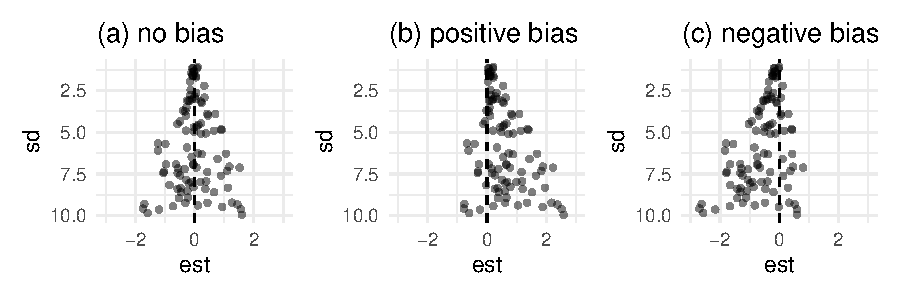
\includegraphics{Draft_RR_files/figure-latex/funnel-plot-1.pdf}
\caption{\label{fig:funnel-plot}Illustrations of funnel plots showing (a) no bias, (b) positive bias, and (c) negative bias in effect sizes. The vertical dashed line represents the meta-analitical mean.}
\end{figure}

\hypertarget{ana-factors}{%
\subsubsection{Analytical and demographic factors affecting effect sizes}\label{ana-factors}}

As a second step, we will investigate the extent to which deviations from the meta-analytical mean by individual standardized effect sizes relate to a series of predictors related to analytical and demographic factors (see below).
The deviation score \(\delta_i\), which serves as the dependent variable in this analysis, will be the \highlight[id=SC, comment = {We might wanna fit a me model. See minutes.}]{difference between the meta-analytical mean} (\(\hat{\eta}\)) and the individual standardized effect size of each analysis (\(\eta_i\)).
We will fit a single Bayesian regression model with \(\delta_i\) as the outcome variable, and the analytical and demographic factors described in the following paragraphs as predictors.

\textbf{Analytical factors}. We will model the effect of the following predictors related to the analytical characteristics of each team's reported analysis:

\begin{itemize}
\tightlist
\item
  \emph{Measure of uniqueness} of individual analyses for the set of predictors in each model.
\item
  \emph{Measure of conservativeness} of the model specification.
\item
  \emph{Number of post-hoc changes to the acoustic measurements} the teams will report to have carried out.
\item
  \emph{Number of models} the teams will report to have run.
\item
  \emph{Major dimension} that has been measured to answer the research question.
\item
  \emph{Temporal window} that the measurement is taken over.
\item
  \emph{Data exclusion}, whether data has been excluded or not.
\end{itemize}

The measure of uniqueness of predictors will be assessed by the Sørensen-Dice Index (SDI, Dice, 1945; Sørensen, 1948).
The SDI is an index typically used in ecology research to compare species composition across sites.
For our purposes, we will treat predictors as species and individual analyses as sites.
The SDI for a pair of analyses \((X, Y)\) can be obtained using the following formula:

\[\text{SDI} = \frac{2|X \cap Y|}{|X|+|Y|}\]

where \(|X \cap Y|\) is the number of variables common to both models, and \(|X|+|Y|\) is the sum of the number of variables that occur in each model.

In order to generate a unique SDI for each analysis team, we will calculate the average of all pairwise SDIs for all pairs of analyses using the \texttt{beta.pair()} function in the betapart R package (Baselga et al.~2018).

The major measurement dimension of each analysis will be categorized according to the following possible groups: duration, amplitude, fundamental frequency, other spectral properties (e.g.~frequency center of gravity, harmonics difference, etc.), other measures (e.g.~principal components, vowel dispersion, etc.)
The temporal window that the measurement is taken over is defined by the target linguistic unit.
We assume the following relevant linguistic units: segment, syllable, word, phrase.

\textbf{Demographic factors}. We will include the following demographic factors about the \highlight[id=SC, comment = {How do we do this, since we will have a score per individual rather than per team?}]{analysis} teams:

\begin{itemize}
\tightlist
\item
  \emph{Research experience} as the elapsed time from PhD award (negative values will indicate that the person is a student or graduate student).
\item
  \emph{Initial belief} in the presence of an effect of atypical noun-adjective pairs on acoustics, as answered during the intake questionnaire.
\end{itemize}

We will publicly archive all relevant data, code, and materials on the Open Science Framework (\url{https://osf.io/3bmcp/}).
Archived data will include the original data sets distributed to all analysts, any edited versions of the data analyzed by individual groups, and the data we analyze with our meta-analyses, which include the effect sizes derived from separate analyses, the statistics describing variation in model structure among analysis teams, and the anonymized answers to our surveys of analysts and peer reviewers.
Similarly, we will archive both the analysis code used for each individual analysis and the code from our meta-analyses.
We will also archive copies of our survey instruments from analysts and peer reviewers.

Our rules for excluding data from our study are as follows.
We will exclude from our synthesis any individual analysis submitted after we have completed peer review or those unaccompanied by analysis files that allow us to understand what the analysts did.
We will also exclude any individual analysis that does not produce an outcome that can be interpreted as an answer to our primary question.

\hypertarget{step-6-collaborative-write-up-of-manuscript}{%
\subsection{Step 6: Collaborative Write-Up of Manuscript}\label{step-6-collaborative-write-up-of-manuscript}}

Analysts and initiating authors will discuss the limitations, results, and implications of the study and collaborate on writing the final manuscript for review as a stage-2 Registered Report.

\newpage

\hypertarget{references}{%
\section{References}\label{references}}

\begingroup
\setlength{\parindent}{-0.5in}
\setlength{\leftskip}{0.5in}

\hypertarget{refs}{}
\begin{CSLReferences}{1}{0}
\leavevmode\hypertarget{ref-arts2011overspecification}{}%
Arts, A., Maes, A., Noordman, L. G., \& Jansen, C. (2011). Overspecification in written instruction. \emph{Linguistics}, \emph{49}(3), 555--574.

\leavevmode\hypertarget{ref-botvinik2020variability}{}%
Botvinik-Nezer, R., Holzmeister, F., Camerer, C. F., Dreber, A., Huber, J., Johannesson, M., \ldots{} others. (2020). Variability in the analysis of a single neuroimaging dataset by many teams. \emph{Nature}, 1--7.

\leavevmode\hypertarget{ref-box1976science}{}%
Box, G. E. (1976). Science and statistics. \emph{Journal of the American Statistical Association}, \emph{71}(356), 791--799.

\leavevmode\hypertarget{ref-camerer2018evaluating}{}%
Camerer, C. F., Dreber, A., Holzmeister, F., Ho, T.-H., Huber, J., Johannesson, M., \ldots{} others. (2018). Evaluating the replicability of social science experiments in nature and science between 2010 and 2015. \emph{Nature Human Behaviour}, \emph{2}(9), 637--644. \url{https://doi.org/10.1038/s41562-018-0399-z}

\leavevmode\hypertarget{ref-de2014thought}{}%
De Groot, A. D. (2014). \emph{Thought and choice in chess} (Vol. 4). Walter de Gruyter GmbH \& Co KG.

\leavevmode\hypertarget{ref-degen2020redundancy}{}%
Degen, J., Hawkins, R. D., Graf, C., Kreiss, E., \& Goodman, N. D. (2020). When redundancy is useful: A bayesian approach to {``overinformative''} referring expressions. \emph{Psychological Review}.

\leavevmode\hypertarget{ref-dice1945}{}%
Dice, L. R. (1945). Measures of the amount of ecologic association between species. \emph{Ecology}, \emph{26}(3), 297--302.

\leavevmode\hypertarget{ref-egger1997}{}%
Egger, M., Smith, G. D., Schneider, M., \& Minder, C. (1997). Bias in meta-analysis detected by a simple, graphical test. \emph{British Medical Journal}, \emph{315}, 629--634.

\leavevmode\hypertarget{ref-fischhoff1975hindsight}{}%
Fischhoff, B. (1975). Hindsight is not equal to foresight: The effect of outcome knowledge on judgment under uncertainty. \emph{Journal of Experimental Psychology: Human Perception and Performance}, \emph{1}(3), 288.

\leavevmode\hypertarget{ref-flake2019}{}%
Flake, J. K., \& Fried, E. I. (2019). Measurement schmeasurement: Questionable measurement practices and how to avoid them. Pre-print available at PsyArXiv.

\leavevmode\hypertarget{ref-foulkes2006}{}%
Foulkes, P., \& Docherty, G. (2006). The social life of phonetics and phonology. \emph{Journal of Phonetics}, \emph{34}(4), 409--438.

\leavevmode\hypertarget{ref-gatt2013we}{}%
Gatt, A., Gompel, R. P. van, Deemter, K. van, \& Krahmer, E. (2013). Are we bayesian referring expression generators. Cognitive Science Society.

\leavevmode\hypertarget{ref-gelman2014statistical}{}%
Gelman, A., \& Loken, E. (2014). The statistical crisis in science: Data-dependent analysis--a" garden of forking paths"--explains why many statistically significant comparisons don't hold up. \emph{American Scientist}, \emph{102}(6), 460--466.

\leavevmode\hypertarget{ref-gordon2017acoustic}{}%
Gordon, M., \& Roettger, T. (2017). Acoustic correlates of word stress: A cross-linguistic survey. \emph{Linguistics Vanguard}, \emph{3}(1), 1--11.

\leavevmode\hypertarget{ref-grice1975logic}{}%
Grice, H. P. (1975). Logic and conversation. In \emph{Speech acts} (pp. 41--58). Brill.

\leavevmode\hypertarget{ref-hawkins2004influence}{}%
Hawkins, S., \& Nguyen, N. (2004). Influence of syllable-coda voicing on the acoustic properties of syllable-onset /l/ in {E}nglish. \emph{Journal of Phonetics}, \emph{32}(2), 199--231.

\leavevmode\hypertarget{ref-jongman2000acoustic}{}%
Jongman, A., Wayland, R., \& Wong, S. (2000). Acoustic characteristics of english fricatives. \emph{The Journal of the Acoustical Society of America}, \emph{108}(3), 1252--1263.

\leavevmode\hypertarget{ref-knight2000}{}%
Knight, K. (2000). \emph{Mathematical statistics}. Chapman; Hall, New York.

\leavevmode\hypertarget{ref-koole2012rewarding}{}%
Koole, S. L., \& Lakens, D. (2012). Rewarding replications: A sure and simple way to improve psychological science. \emph{Perspectives on Psychological Science}, \emph{7}(6), 608--614.

\leavevmode\hypertarget{ref-ladd2008intonational}{}%
Ladd, D. R. (2008). \emph{Intonational phonology}. Cambridge University Press.

\leavevmode\hypertarget{ref-lau2006}{}%
Lau, J., Ioannidis, J. P. A., Terrin, N., Schmid, C. H., \& Olkin, I. (2006). The case of the misleading funnel plot. \emph{British Medical Journal}, \emph{333}(7568), 597--600.

\leavevmode\hypertarget{ref-light1984}{}%
Light, R. J., \& Pillemer, D. B. (1984). \emph{Summing up; the science of reviewing research}. Cambridge, MA (USA) Harvard Univ. Press.

\leavevmode\hypertarget{ref-lisker1977rapid}{}%
Lisker, L. (1977). Rapid versus rabid: A catalogue of acoustic features that may cue the distinction. \emph{The Journal of the Acoustical Society of America}, \emph{62}(S1), S77--S78.

\leavevmode\hypertarget{ref-lisker1986voicing}{}%
Lisker, L. (1986). {``Voicing''} in {E}nglish: A catalogue of acoustic features signaling /b/ versus /p/ in trochees. \emph{Language and Speech}, \emph{29}(1), 3--11.

\leavevmode\hypertarget{ref-nickerson1998confirmation}{}%
Nickerson, R. S. (1998). Confirmation bias: A ubiquitous phenomenon in many guises. \emph{Review of General Psychology}, \emph{2}(2), 175--220.

\leavevmode\hypertarget{ref-nosek2014method}{}%
Nosek, B. A., \& Lakens, D. (2014). A method to increase the credibility of published results. \emph{Social Psychology}, \emph{45}(3), 137--141.

\leavevmode\hypertarget{ref-ogden2004}{}%
Ogden, R. (2004). Non-modal voice quality and turn-taking in {F}innish. \emph{Sound Patterns in Interaction: Cross-Linguistic Studies from Conversation}, 29--62.

\leavevmode\hypertarget{ref-open2015estimating}{}%
Open Science Collaboration. (2015). Estimating the reproducibility of psychological science. \emph{Science}, \emph{349}(6251). \url{https://doi.org/10.1126/science.aac4716}

\leavevmode\hypertarget{ref-paraboni2007generating}{}%
Paraboni, I., Van Deemter, K., \& Masthoff, J. (2007). Generating referring expressions: Making referents easy to identify. \emph{Computational Linguistics}, \emph{33}(2), 229--254.

\leavevmode\hypertarget{ref-roettger2019researcher}{}%
Roettger, T. B. (2019). Researcher degrees of freedom in phonetic research. \emph{Laboratory Phonology: Journal of the Association for Laboratory Phonology}, \emph{10}(1).

\leavevmode\hypertarget{ref-rotello2015more}{}%
Rotello, C. M., Heit, E., \& Dubé, C. (2015). When more data steer us wrong: {R}eplications with the wrong dependent measure perpetuate erroneous conclusions. \emph{Psychonomic Bulletin \& Review}, \emph{22}(4), 944--954.

\leavevmode\hypertarget{ref-rubio2016redundant}{}%
Rubio-Fernández, P. (2016). How redundant are redundant color adjectives? An efficiency-based analysis of color overspecification. \emph{Frontiers in Psychology}, \emph{7}, 153.

\leavevmode\hypertarget{ref-sedivy2003pragmatic}{}%
Sedivy, J. C. (2003). Pragmatic versus form-based accounts of referential contrast: Evidence for effects of informativity expectations. \emph{Journal of Psycholinguistic Research}, \emph{32}(1), 3--23.

\leavevmode\hypertarget{ref-silberzahn2018many}{}%
Silberzahn, R., Uhlmann, E. L., Martin, D. P., Anselmi, P., Aust, F., Awtrey, E., \ldots{} others. (2018). Many analysts, one data set: Making transparent how variations in analytic choices affect results. \emph{Advances in Methods and Practices in Psychological Science}, \emph{1}(3), 337--356.

\leavevmode\hypertarget{ref-simmons2011false}{}%
Simmons, J. P., Nelson, L. D., \& Simonsohn, U. (2011). False-positive psychology: Undisclosed flexibility in data collection and analysis allows presenting anything as significant. \emph{Psychological Science}, \emph{22}(11), 1359--1366.

\leavevmode\hypertarget{ref-starns2019assessing}{}%
Starns, J. J., Cataldo, A. M., Rotello, C. M., Annis, J., Aschenbrenner, A., Bröder, A., \ldots{} Wilson, J. (2019). Assessing theoretical conclusions with blinded inference to investigate a potential inference crisis. \emph{Advances in Methods and Practices in Psychological Science}, \emph{2}(4), 335--349.

\leavevmode\hypertarget{ref-sterling1959publication}{}%
Sterling, T. D. (1959). Publication decisions and their possible effects on inferences drawn from tests of significance---or vice versa. \emph{Journal of the American Statistical Association}, \emph{54}(285), 30--34.

\leavevmode\hypertarget{ref-sterne2005}{}%
Sterne, J. A. C., Becker, B. J., \& Egger, M. (2005). The funnel plot. In H. R. Rothstein, A. J. Sutton, \& M. Borenstein (Eds.), \emph{Publication bias in meta-analysis: Prevention, assessment and adjustments} (pp. 75--98). Wiley Online Library.

\leavevmode\hypertarget{ref-sorensen1948}{}%
Sørensen, T. (1948). A method of establishing groups of equal amplitude in plant sociology based on similarity of species and its application to analyses of the vegetation on {D}anish commons. \emph{Kongelige Danske Videnskabernes Selskab}, \emph{5}(4), 1--34.

\leavevmode\hypertarget{ref-tukey1977exploratory}{}%
Tukey, J. W. (1977). \emph{Exploratory data analysis} (Vol. 2). Reading, MA.

\leavevmode\hypertarget{ref-tversky1974judgment}{}%
Tversky, A., \& Kahneman, D. (1974). Judgment under uncertainty: Heuristics and biases. \emph{Science}, \emph{185}(4157), 1124--1131.

\leavevmode\hypertarget{ref-van2005speech}{}%
Van Heuven, V. J., \& Van Zanten, E. (2005). Speech rate as a secondary prosodic characteristic of polarity questions in three languages. \emph{Speech Communication}, \emph{47}(1-2), 87--99.

\leavevmode\hypertarget{ref-wagenmakers2012agenda}{}%
Wagenmakers, E.-J., Wetzels, R., Borsboom, D., Maas, H. L. van der, \& Kievit, R. A. (2012). An agenda for purely confirmatory research. \emph{Perspectives on Psychological Science}, \emph{7}(6), 632--638.

\leavevmode\hypertarget{ref-westerbeek2015stored}{}%
Westerbeek, H., Koolen, R., \& Maes, A. (2015). Stored object knowledge and the production of referring expressions: The case of color typicality. \emph{Frontiers in Psychology}, \emph{6}, 935.

\leavevmode\hypertarget{ref-white2009}{}%
White, L., Payne, E., \& Mattys, S. L. (2009). Rhythmic and prosodic contrast in {V}enetan and {S}icilian {I}talian. In M. Vigario, S. Frota, \& M. J. Freitas (Eds.), \emph{Phonetics and phonology: Interactions and interrelations} (pp. 137--158). Amsterdam: John Benjamins.

\leavevmode\hypertarget{ref-wicherts2006poor}{}%
Wicherts, J. M., Borsboom, D., Kats, J., \& Molenaar, D. (2006). The poor availability of psychological research data for reanalysis. \emph{American Psychologist}, \emph{61}(7), 726.

\leavevmode\hypertarget{ref-winter2014spoken}{}%
Winter, B. (2014). Spoken language achieves robustness and evolvability by exploiting degeneracy and neutrality. \emph{BioEssays}, \emph{36}(10), 960--967.

\end{CSLReferences}

\endgroup


\end{document}
